%%%%%%%%%%%%%%%%%%%%%%%%%%%%%%%%%%%%%%%%%%%%%%%%%%%%%%%%%%%%%%%
%%%  NEG 
%%%%%%%%%%%%%%%%%%%%%%%%%%%%%%%%%%%%%%%%%%%%%%%%%%%%%%%%%%%%%%%

% For submission redefine \rmrk \hrefl \hidea

\documentclass[aps,pre,floats,floatfix,twocolumn]{revtex4}
%\documentclass[fleqn,10pt]{wlscirep}

% special 
\usepackage{ifthen}
\usepackage{ifpdf}
\usepackage{color}

\ifpdf
\usepackage{graphicx}
\usepackage{epstopdf}
\else
\usepackage{graphicx}
\usepackage{epsfig}
\fi
\graphicspath{{./Figs/}{./}}
\graphicspath{{/Users/danielhurowitz/PROJ/NHR/Figs/}{/Users/danielhurowitz/PROJ/NEG/Figs/figs_for_paper/}{./}{../}}

% fonts
\usepackage{latexsym}
\usepackage{amsmath}
\usepackage{amssymb}
\usepackage{bm}
\usepackage{wasysym}

\usepackage{mathptmx}
\DeclareSymbolFont{epsilon}{OML}{ntxmi}{m}{it}
\DeclareMathSymbol{\epsilon}{\mathord}{epsilon}{"0F}

\usepackage{hyperref}

% Standard symbols 
\newcommand{\sinc}{\mbox{sinc}}
\newcommand{\const}{\mbox{const}}
\newcommand{\trc}{\mbox{trace}}
\newcommand{\intt}{\int\!\!\!\!\int }
\newcommand{\ointt}{\int\!\!\!\!\int\!\!\!\!\!\circ\ }
\newcommand{\ar}{\mathsf r}
\newcommand{\im}{\mbox{Im}}
\newcommand{\re}{\mbox{Re}}

% Special symbols
\newcommand{\mass}{\mathsf{m}} 
\newcommand{\Mass}{\mathsf{M}} 

% Math constractions
\newcommand{\tbox}[1]{\mbox{\tiny #1}}
\newcommand{\bmsf}[1]{\bm{\mathsf{#1}}} 
\newcommand{\amatrix}[1]{\begin{matrix} #1 \end{matrix}} 
\newcommand{\eexp}[1]{\mathrm{e}^{#1}}
\newcommand{\pd}[2]{\frac{\partial #1}{\partial #2}}
\newcommand{\bra}[1]{\left\langle #1 \right|}
\newcommand{\ket}[1]{\left| #1 \right\rangle}
\newcommand{\braket}[1]{ \left\langle #1 \right\rangle}
\newcommand{\Braket}[2]{ \left\langle #1 \middle| #2 \right\rangle}
\newcommand{\BraKet}[3]{ \left\langle #1 \middle| #2 \middle| #3 \right\rangle}
\newcommand{\avg}[1]{\left\langle #1 \right\rangle}
\newcommand{\ola}{\protect\overleftarrow}
\newcommand{\ora}{\protect\overrightarrow}

% Equations
\newcommand{\be}[1]{\begin{eqnarray}\ifthenelse{#1=-1}{\nonumber}{\ifthenelse{#1=0}{}{\label{e#1}}}}
\newcommand{\beq}{\begin{eqnarray}}
\newcommand{\eeq}{\end{eqnarray}} 

% Text arrangement
\newcommand{\hide}[1]{}

\newcommand{\Eq}[1]{\textcolor{blue}{{equation}\!~(\ref{#1})}} 
\newcommand{\Ap}[1]{\textcolor{blue}{{appendix}\!~(\ref{#1})}} 
\newcommand{\Sec}[1]{\textcolor{blue}{{section}\!~(\ref{#1})}} 
\newcommand{\Fig}[1]{\textcolor{blue}{Fig.}\!\!~\ref{#1}}
\newcommand{\sect}[1]{{\bf #1.-- }}
\newcommand{\drawline}{\begin{picture}(500,1)\line(1,0){500}\end{picture}}
\newcommand{\bitem}{$\bullet$ \ \ \ }
\newcommand{\Cn}[1]{\begin{center} #1 \end{center}}
%\renewcommand{\cite}[1]{\textcolor{blue}{[\onlinecite{#1}}]} %{[\onlinecite{#1}]} 



% temporary turn off figures
%\renewcommand{\includegraphics}[2][]{{\color{blue} \hspace{5mm} --FIGURE-- \hspace{5mm} }}

%\newcommand{\rmrk}[1]{{#1}}     %{\textcolor[rgb]{0.6,0,0.1}{#1}}
\newcommand{\rmrk}[1]{{\color[rgb]{0.6,0,0.1} #1}}
\newcommand{\hrefl}[1]    {\href{#1}{[link]}}
\newcommand{\hidea}[1]{{#1}}


%%%%%%%%%%%%%%%%%%%%%%%%%%%%%%%%%%%%%%%%%%%%%%%%%%%%%%%%%%%%%%%%%%%%%%%%%%%%%%%%%%%%%%%%%%
%%%%%%%%%%%%%%%%%%%%%%%%%%%%%%%%%%%%%%%%%%%%%%%%%%%%%%%%%%%%%%%%%%%%%%%%%%%%%%%%%%%%%%%%%%
\begin{document}
\[\title{Percolation, sliding, localization and relaxation in topologically closed circuits}

\author{Daniel Hurowitz, Doron Cohen}

\affiliation{Department of Physics, Ben-Gurion University of the Negev, Beer-Sheva, Israel}

%%%%%%%%%%%%%%%%%%%%%%%%%%%%%%%%%%%%%%%%%%%%%%%%%%%%%%%%%%%%%%%%%%%%%%%%%%%%%%%%%%%%%%%%%%
%%%%%%%%%%%%%%%%%%%%%%%%%%%%%%%%%%%%%%%%%%%%%%%%%%%%%%%%%%%%%%%%%%%%%%%%%%%%%%%%%%%%%%%%%%

\maketitle

%\begin{abstract}
{\bf
The ``glassy" version of {\em random walk on disordered lattice}  
features a percolation-related crossover to variable-range-hopping,
or to sub-diffusion in one-dimension.  
The more general problem of {\em random walk in random environment}, 
where transition rates are allowed to be asymmetric, 
has been explored by Sinai, Derrida, and followers.  
It turns out that for any small amount of disorder 
an unbiased spreading in one-dimension becomes sub-diffusive,  
while for bias that exceeds a finite threshold there 
is a {\em sliding transition}, leading to a non-zero drift velocity.
%
In the present study we explore the implications of the percolation and sliding transitions 
for the relaxation modes of a topologically closed circuit. 
A complementary question regarding  the ``delocalization" of eigenstates 
of non-hermitian Hamiltonians has been addressed by Hatano, Nelson, and followers. 
But we show that for a conservative random-walk dynamics 
the implied spectral properties are dramatically different.
}
%\end{abstract}


The original version of Einstein's Brownian motion problem
is essentially equivalent to the analysis of a simple {\em random walk}. 
The more complicated version is {\em random walk on a disordered lattice},  
which is like a resistor-network problem, 
involving a percolation-like transition \cite{Alexander}.  
The latter has diverse applications, e.g. 
in the context of ``glassy" electron dynamics \cite{ege,egt}. 
%
But more generally one has to consider Sinai's spreading problem \cite{Sinai,odh1,odh3,BouchaudReview}, 
aka {\em random walk in a random environment}, 
that has relevance e.g. for studies in a biophysical context: 
population biology \cite{popbio,popbio2}, pulling pinned polymers and DNA denaturation \cite{DNA1,DNA2} 
and processive molecular motors \cite{fisher1999force,rief2000myosin}.

%
In all these cases the dynamics can be regarded as a stochastic process 
in which a particle hops from site to site.
The rate equation for the site occupation probabilities $\bm{p}  = \{p_n\}$
can be written in matrix notation as 
%
\be{1}
\frac{d\bm{p}}{dt} \ \ = \ \ \bm{W} \bm{p}, 
\eeq
%
involving a matrix ${\bm{W}}$ whose off-diagonal elements 
are the transitions rates ${w_{nm}}$, 
and with diagonal elements ${-\gamma_n}$ such that each column sums to zero.
Assuming near-neighbor hopping the ${\bm{W}}$ matrix takes the form
%
\be{2}
\bm{W} \ \ = \ \ \left[\amatrix{
-\gamma_1   & w_{1,2}   & 0         & ... \\ 
w_{2,1}     & -\gamma_2 & w_{2,3}   & ... \\ 
0           & w_{3,2}   & -\gamma_3 & ... \\
...         & ...       & ...       & ...
}\right]
\eeq 
%
In Einstein's theory $\bm{W}$ is symmetric, 
and all the non-zero rates are the same; 
In the resistor-network problem the rates
have some distribution $P(w)$ that features (see Methods)
%
\be{4}
P(w) \ \propto \ w^{\alpha-1} \ \ \ \ \text{(for small $w$)}
\eeq
%
But in Sinai's problem $\bm{W}$ is allowed to be asymmetric.
Accordingly the rates at the $n$th bond can be written 
as $w_n\eexp{\pm\mathcal{E}_n/2}$ 
for forward  and backward transitions respectively. 
For the purpose of presentation we assume that the stochastic field~$\mathcal{E}$  
is box distributed within ${[s-\sigma,s+\sigma]}$.
We refer to~$s$ as the bias:  
it is the pulling force in the case of depinning polymers and DNA denaturation; 
or the convective flow of bacteria relative to the nutrients in the case of population biology; 
or the affinity of the chemical cycle in the case of molecular motors.

Our interest is in the relaxation dynamics 
of finite $N$-site ring-shaped circuits, 
that are described by the stochastic equation \Eq{e1}.
The $N$~sites might be physical locations in some lattice 
structure, or can represent steps of some chemical-cycle. 
For example, in the Brownian motor context $N$~is the number 
of chemical-reactions required to advance the motor one pace. 
%
We are inspired by the study of of non-Hermitian quantum Hamiltonians 
with regard to vortex depinning in type II superconductors \cite{Hatano1,Hatano2,Shnerb1};   
molecular motors with {\em finite} processivity \cite{brm1,brm2}; 
and related works \cite{Brouwer,Goldsheid,Zee}.
In both examples conservation of probability is violated.  
In the first example the bias is the applied transverse magnetic field;  
and $N$~is the number of defects to which the magnetic vortex can pin.


\sect{Scope} 
In this article we report how the spectral properties of the matrix $\bm{W}$ 
depend on the parameters $(\alpha,\sigma,s)$, as defined after \Eq{e2}. 
These parameters describe respectively the resistor-network disorder, 
the stochastic-field disorder, and the average bias field.    
The eigenvalues $\{-\lambda_k\}$ of $\bm{W}$ are associated 
with the relaxation modes of the system. 
Due to conservation of probability ${\lambda_0=0}$, 
while all the other eigenvalues ${\{\lambda_k\}}$ have positive 
real part, and may have an imaginary part as well. 
Complex eigenvalues imply that the relaxation is not over-damped: 
one would be able to observe an oscillating density during relaxation, 
as demonstrated in \Fig{traj}.    
%
The first row of \Fig{froots} provides some representative spectra.
As the bias~$s$ is increased a complex bubble appears at the bottom 
of the band, implying delocalization of the eigenstates.   
Our results for the complexity threshold~$s_c$ are summarized 
in table \ref{tbl}, and demonstrated in \Fig{figSc}. 
The number of complex eigenvalues grows as a function 
of the bias, as demonstrated in \Fig{figCplxSat},  
but asymptotically only a finite fraction of the spectrum becomes complex. 
%
Our objective below is to explain analytically the 
peculiarities of this delocalization transition, 
to explain how it is affected by the percolation and by the sliding thresholds, 
and to analyze the complexity-saturation effect.  




%%%%%%%%%%%%%%%%%%%%%%%%%%%%%%%
\begin{table*}

\begin{tabular}{|c|c|c|c|l|}
\hline 
Type of disorder & Parameters &  $s_c$ & Remarks & Figure \\ 
\hline
Resistor-network disorder & $\alpha{<}\frac{1}{2}, \ \sigma{=}0$    &  $s_c = \infty$ &  non-percolating &   \\
Resistor-network disorder & $\frac{1}{2}{<}\alpha{<}1, \ \sigma{=}0$   &  $s_c \sim (1/N)$ & residual percolation & \Fig{figSc}b \\
Sparse disorder & $(M/N) \ll 1$ &  $s_c \sim (1/N)$  &  both disorder types  &  \Fig{figSc}a \\
Stochastic field disorder & $\alpha{>}1, \ \sigma{\ne}0$ & $s_c \approx s_{1/2}$ & percolating & \Fig{figCplxSat} \\
\hline
\end{tabular}

\caption{\label{tbl}
{\bf The complexity threshold for different types of disorder}. (Aka delocalization transition). 
We distinguish between resistor network disorder and stochastic field disorder.  
The threshold $s_{1/2}$ reflects the strength~$\sigma$ of the latter. 
It is smaller than the $s_1$~threshold of the sliding transition.    
Note that the thresholds $s_{\mu}$ depend neither on~$N$ nor on~$\alpha$. 
} 

\end{table*}
%%%%%%%%%%%%%%%%%%%%%%%%%%%%%%%




% trajectories 
%%%%%%%%%%%%%%%%%%%%%%%%%%%%%%%
\begin{figure*}
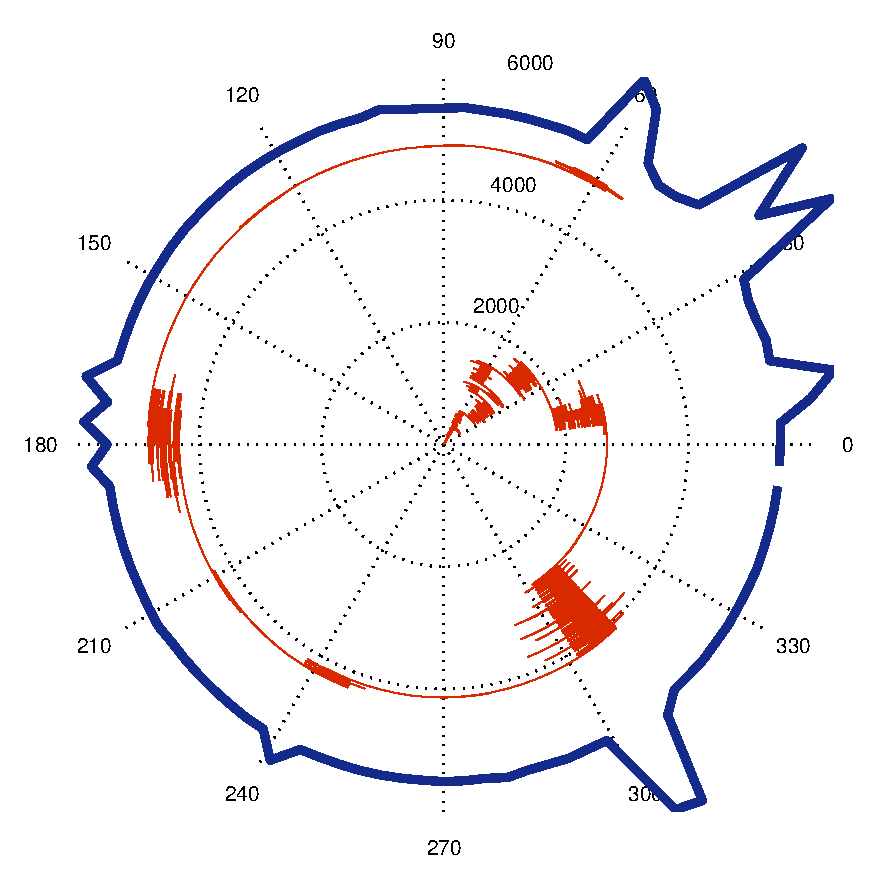
\includegraphics[height=6.5cm]{polar_1_a} \ \ \ \ \ \ \ \  \ \ \ \ \ \ \ \ 
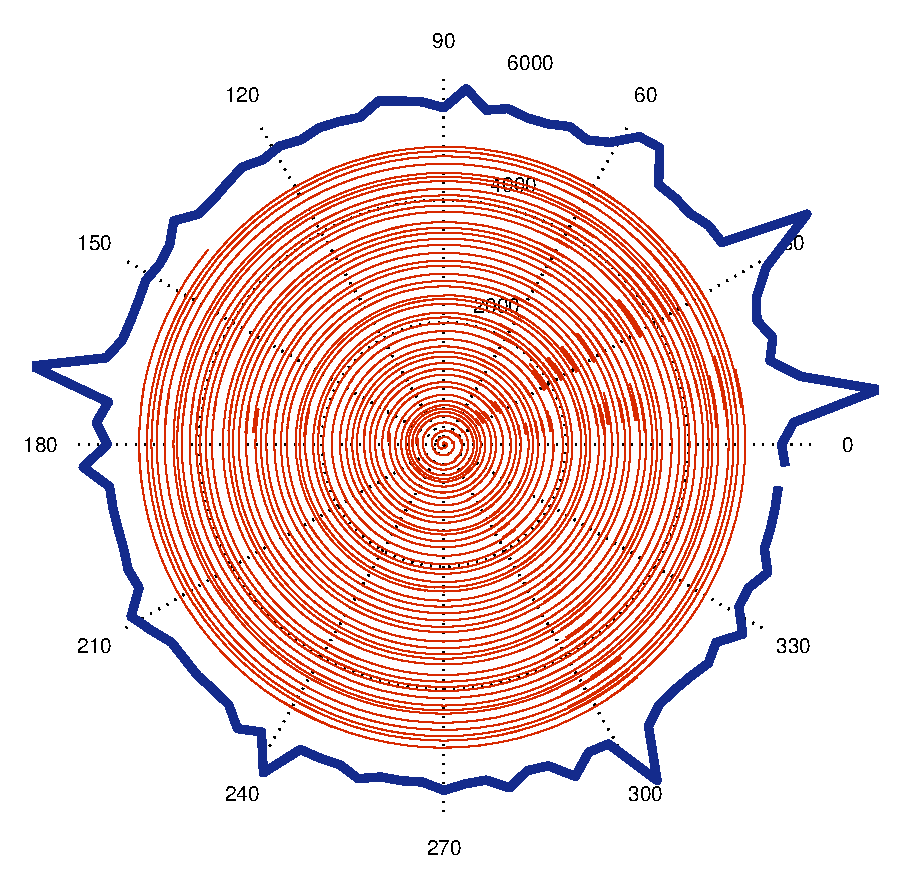
\includegraphics[height=6.5cm]{polar_2_a}

\caption{\label{traj}
{\bf Simulated trajectory of a particle on a disordered-ring.}
The number of sites is $N{=}100$ and the disorder strength is $\sigma{=}5$.
The radial direction is time and the angle is the position. 
For small $s$ (left panel $s{=}0.88$) the dynamics is over-damped, 
while for large $s$ (right panel $s{=}2.97$) the dynamics is under-damped. 
The outer thick line is the steady-state distribution (see Methods). 
% \Ap{Ap12}
}
\end{figure*}



% Complex Plane
%%%%%%%%%%%%%%%%%%%%%%%%%%%%%%%%%%%%%%%%%%%
\begin{figure*}

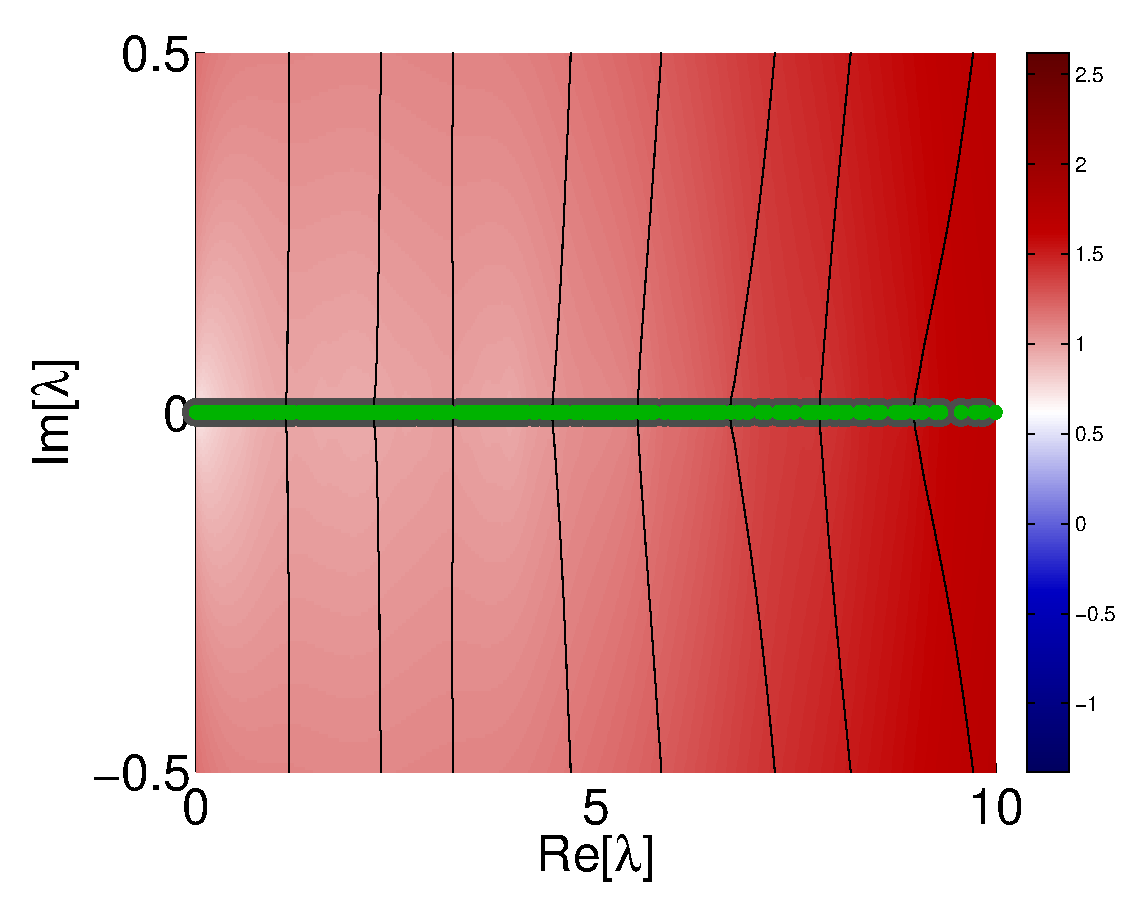
\includegraphics[height=4.5cm]{spectrum_electrostatics1_2}
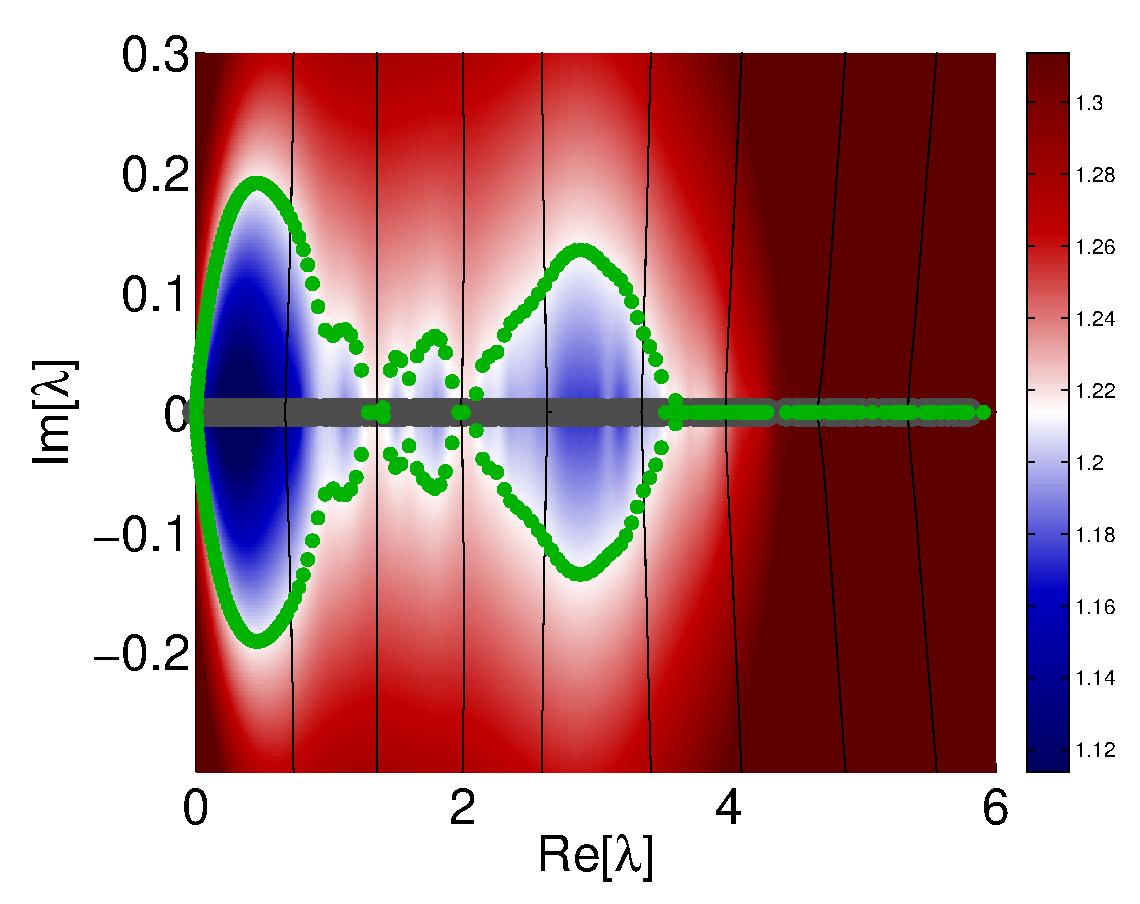
\includegraphics[height=4.5cm]{spectrum_electrostatics1}
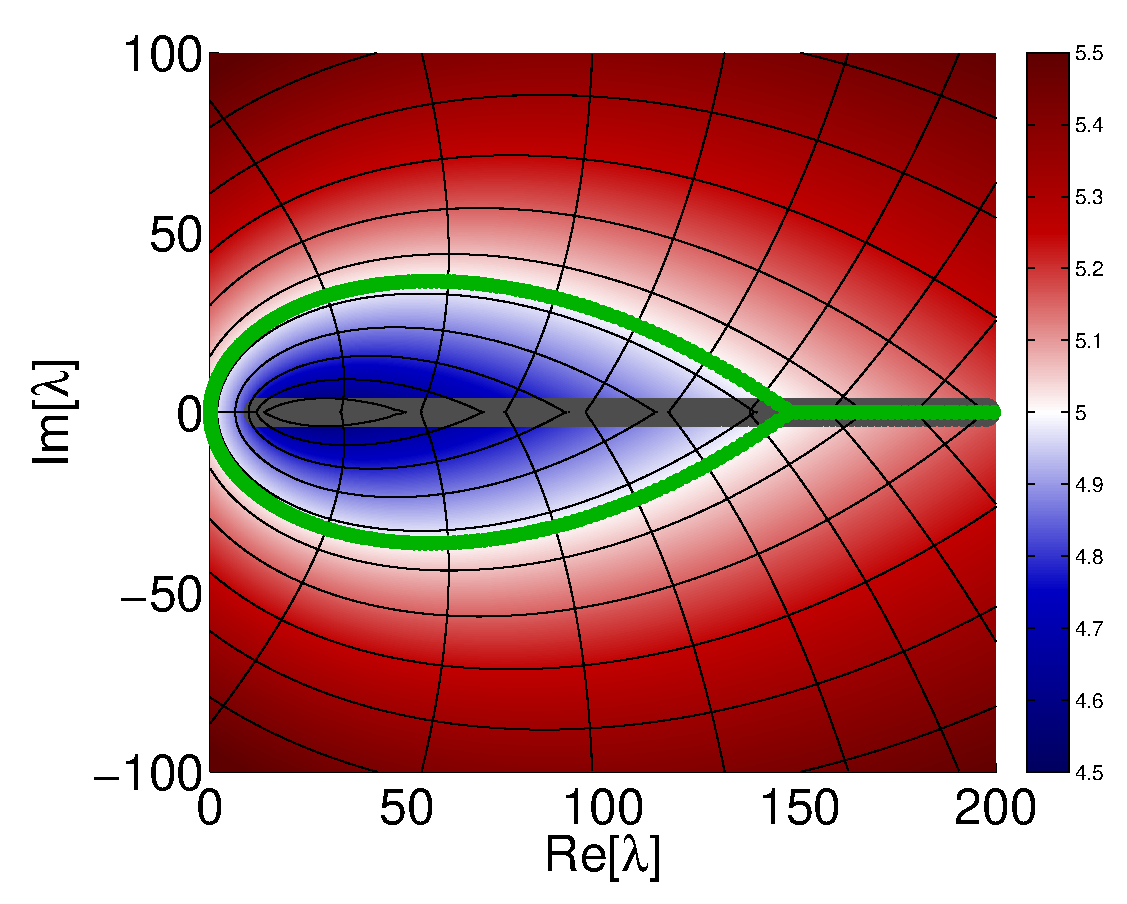
\includegraphics[height=4.5cm]{spectrum_electrostatics2}

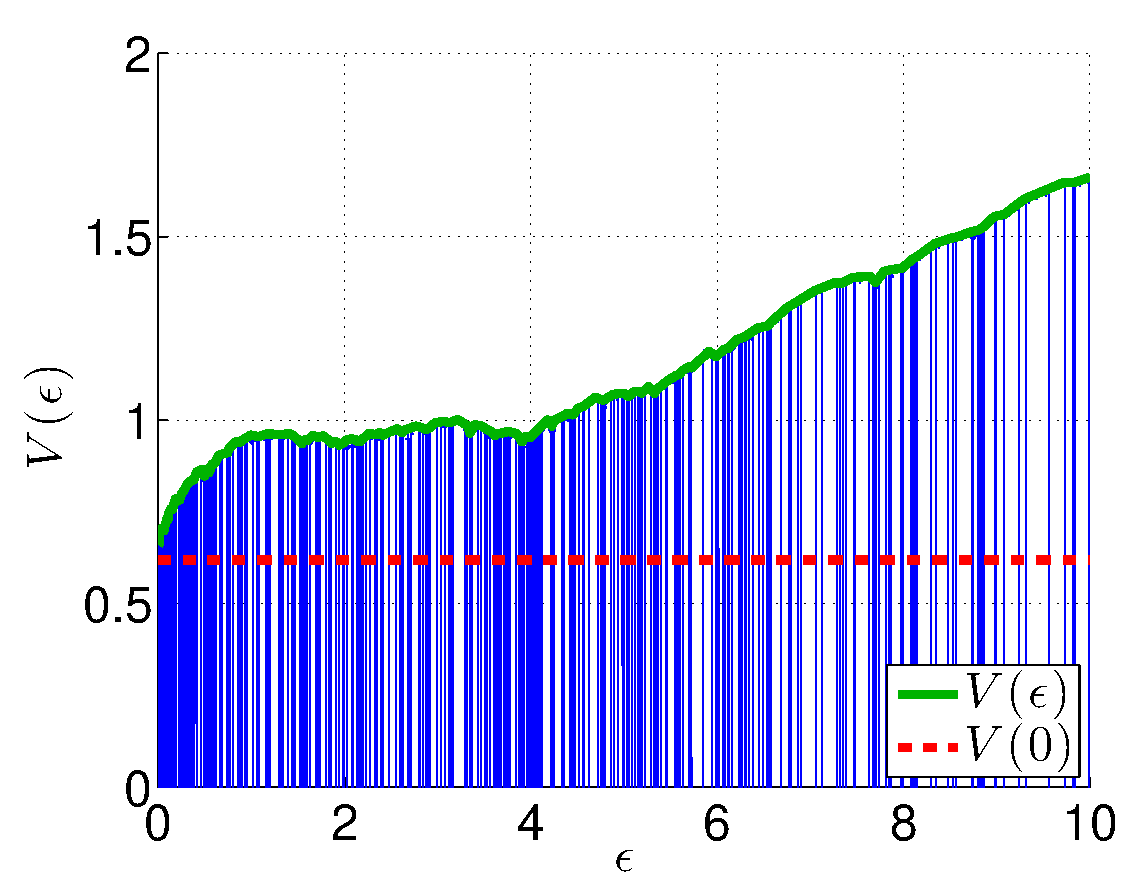
\includegraphics[height=4.5cm]{V_E_1_2b}
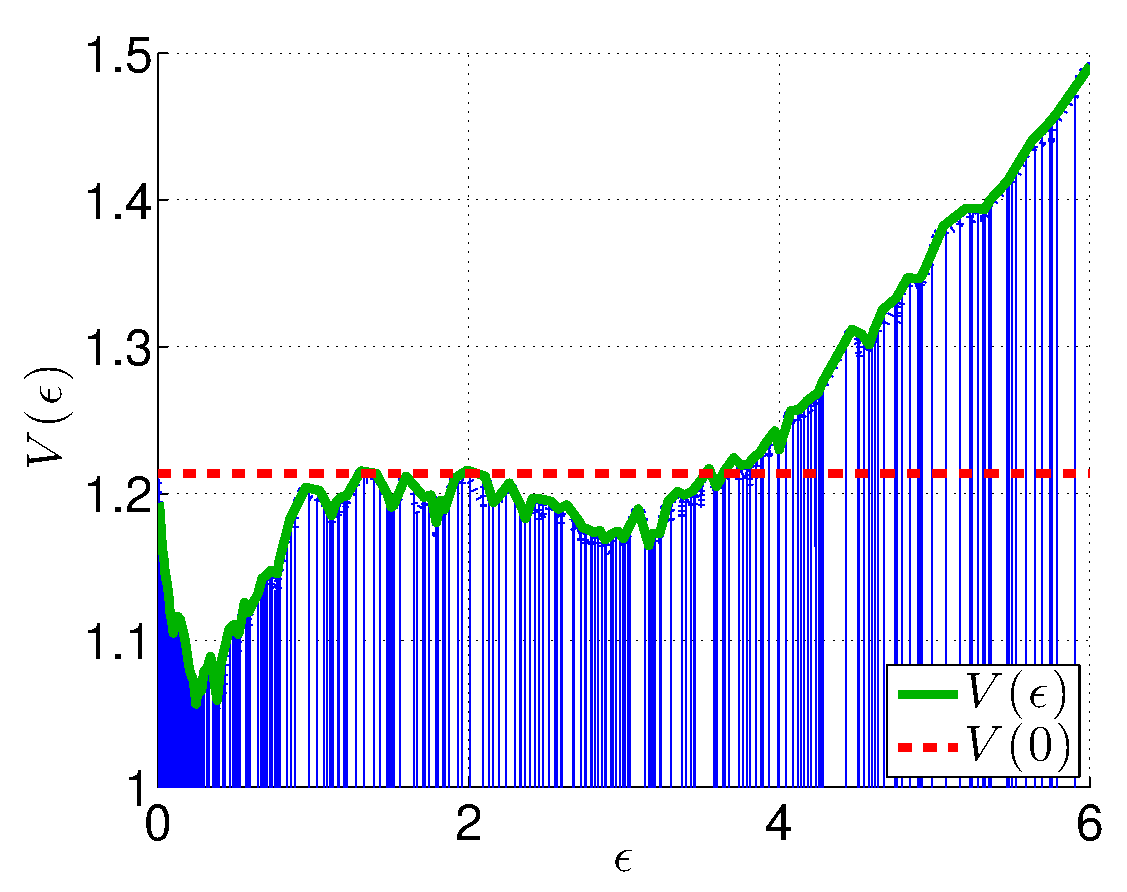
\includegraphics[height=4.5cm]{V_E_1b}
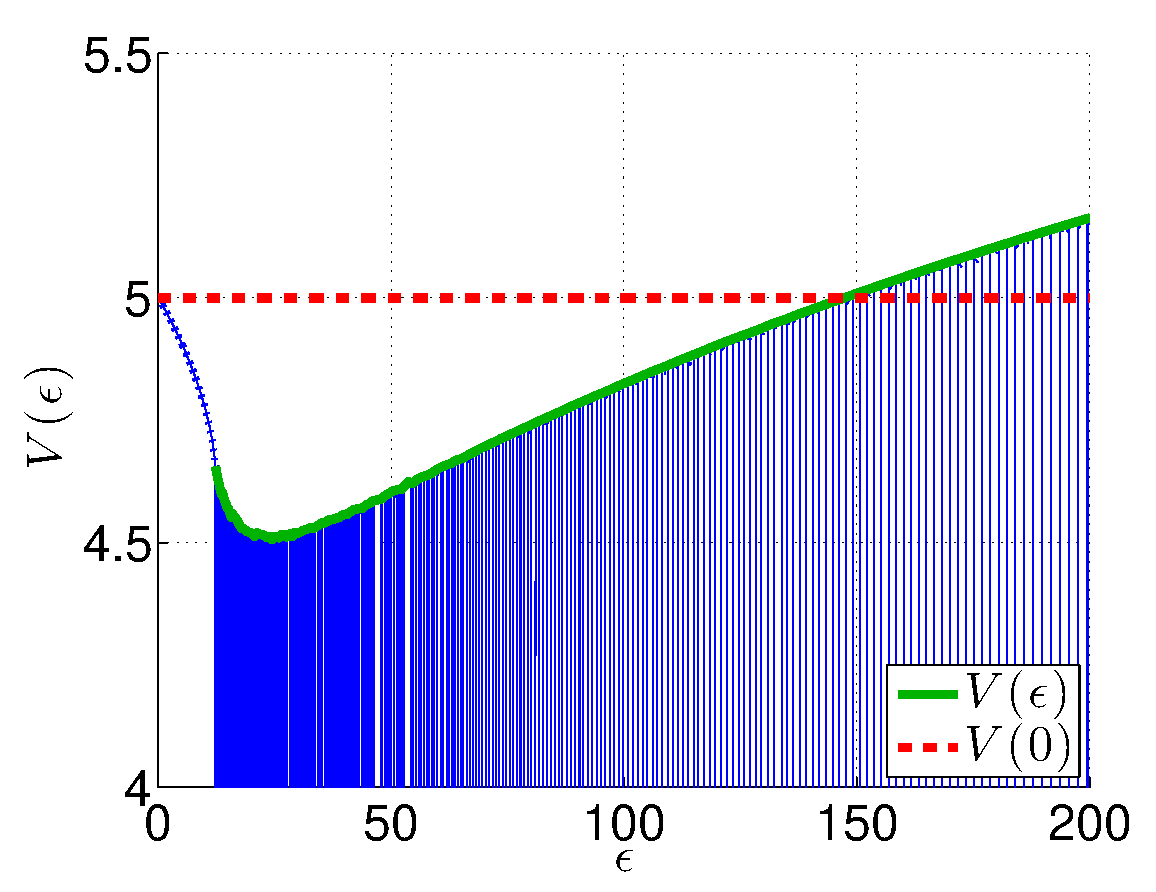
\includegraphics[height=4.5cm]{V_E_2b}

\caption{\label{froots} 
{\bf The emergence of complexity in the relaxation spectrum.} 
The upper panels display representative examples of relaxation spectra.
The $\{\lambda_k\}$ are indicated by green points in the complex plane. 
The ring has $N{=}500$ sites with $\sigma{=}5$, 
and (from left to right) ${s=1.24, 2.43, 10}$. 
The calculated threshold values are ${s_{1/2}=1.77}$ and ${s_1=2.7}$ and ${s_{\infty}=5}$.
In the left hand column ${s<s_{1/2}}$ and the spectrum is real.
In the middle column ${s_{1/2} < s < s_{\infty}}$ and the spectrum is  
with several complex bubbles separated by real segments. 
In the right column  ${s>s_{\infty}}$ and the real spectrum has a gap, 
while the complex spectrum is a fully developed complex bubble, 
tangent to the origin (no gap). 
%
The ``electrostatic field" that is associated with the secular equation 
is represented by a few field-lines, while the background color provides 
visualization of the corresponding electrostatic potential. 
The spectrum is obtained by looking  for the intersections 
of the field lines with the equipotential line ${V(z)=V(0)}$ 
that goes through the origin (indicated in white). 
%
The lower panels plot the potential $V(\epsilon)$ along the real axis. 
The horizontal dashed line is~$V(0)$. 
}
\end{figure*}




%%%%%%%%%%%%%%%%%%%%%%%
\sect{Stochastic spreading}
%
We first consider an opened ring, namely a disordered chain. 
The asymmetry can be gauged away, and $\bm{W}$ becomes similar 
to a symmetric matrix~$\bm{H}$ (see Methods). 
The statistics of its off-diagonal elements 
is characterized by~$\alpha$, 
while the statistics of the diagonal elements 
is also affected by~$\sigma$ and~$s$.   
The eigenvalues $\{-\epsilon_k\}$ of $\bm{H}$ are real.
In the absence of disorder they form a band ${[\epsilon_s,\epsilon_{\infty}]}$
where ${\epsilon_{s,\infty}=2[\cosh(s/2)\mp1]}$. 
%
For sparse disorder with $M$ ($\ll N$) disordered bonds, 
a few additional isolated eigenvalues might appear 
in the gap ${[0,\epsilon_s]}$.
%
With full disorder it is possible to get a gapless spectrum. 
This is the case for Gaussian white-noise stochastic-field disorder 
as analyzed in \cite{odh3}. %see \Ap{A9}.
In this case there is an analytical expression 
for the spectral density in terms of Bessel functions.
The expression features 
%
\be{3}
\rho(\epsilon) \ \propto \ \epsilon^{\mu-1} \ \ \ \ \text{(for small $\epsilon$)}
\eeq
%
with no gap. 
The exponent is related to the bias via ${s=(1/2) \sigma^2 \mu}$. 
%
In the present work we assume the more physically appealing log-box 
disorder for which (see Methods)
%
\be{5}
s \ = \ s_{\mu} \ = \ \frac{1}{\mu} \ln\left( \frac{\sinh (\sigma\mu)}{\sigma\mu} \right)
\eeq
%
Unlike Gaussian disorder the range of possible rates is bounded,  
and we see that a finite threshold ${s_{\infty}=\sigma}$ is deduced.
For ${s>s_{\infty}}$ a gap opens up. 
%
Using the above spectral properties it is deduced that the  
spreading of a distribution along an infinite chain 
goes like $x\sim t^{\mu}$ for ${s<s_1}$, 
while for $s>s_1$ we have a non-zero drift velocity.
This is known as the ``sliding transition".
As for the second moment, for ${\mu<1/2}$ 
the diffusion coefficient is zero. 

The introduction of resistor-network-disorder modifies 
the spectral density at higher energies,
see \Fig{fdos} for illustration. 
For ${\alpha>1}$, in the absence of bias, 
the continuum-limit approximation features ${\mu=1/2}$.
This reflects a normal diffusive behavior 
as in Einstein's theory of Brownian motion. 
Below the percolation threshold, namely for ${\alpha<1}$,
normal diffusion is suppressed, 
and the spectral exponent is ${\mu=\alpha/(1{+}\alpha)<1/2}$. 
But for large bias, the diagonal disorder in~$\bm{H}$ dominates,  
leading to trivially localized eigenstates. 
Hence for large bias we simply have ${\mu=\alpha}$
irrespective of the percolation aspect.  


%%%%%%%%%%%%%%%%%%%%%%%
\sect{Relaxation}
%
We close an $N$-site chain into a ring. 
The ring is characterized by its so-called affinity, 
%
\be{18}
S_{\circlearrowleft} \ \ \equiv \ \ N \, s
\eeq 
%
Now a topological aspect is added to the problem, 
and one wonders what are the relaxation modes of the system. 
%
The starting point of our analysis is the secular 
equation for the eigenvalues of $\bm{W}$.
Assuming that we already know what are the eigenvalues 
of the associated symmetric matrix $\bm{H}$,    
the secular equation takes the form \cite{det1} 
%
\be{20}
\prod_k \left(\frac{z+\epsilon_k(s)}{\overline{w}}\right) \ \ = \ \ 2\left[\cosh\left(\frac{S_{\circlearrowleft}}{2}\right)-1\right]
\eeq
%
where ${\overline{w}}$ is the geometric average of all the rates.
The bias~$s$ affects both the $\epsilon_k$ and the right hand side.
%
This equation has been analyzed in \cite{Shnerb1} 
in the case of a non-conservative matrix~$\bm{W}$ 
whose diagonal elements $\gamma_n$ are {\em fixed}, 
hence the $\epsilon_k(s)$ there do not depend on~$s$. 
Consequently, as~$s$ of \Eq{e18}) is increased beyond 
a threshold value $s_{c}$, the eigenvalues in the middle 
of the spectrum become complex. 
As~$s$ is further increased beyond some higher threshold value, 
the entire spectrum becomes complex. 
As already stated in the introduction, this is not the scenario 
that is observed for our conservative model.
Furthermore we want to clarify how the percolation 
and sliding thresholds are reflected.

Already at this stage one should be aware of the immediate 
implications of conservativity. First of all ${z=\lambda_0=0}$ 
should be a root of the secular equation. 
The associated eigenstate is the non-equilibrium steady state (NESS), 
which is an extended state (see Methods). 
In fact it follows that the localization length has 
to diverge as ${\lambda\rightarrow0}$. 
This is in essence the difference between the 
conventional Anderson model (Lifshitz tails at the band floor) 
and the Debye model (phonons at the band floor). 
It is the latter picture that applies in the 
case of a conservative model.    



% Sc vs N/M
% Sc vs alpha
%%%%%%%%%%%%%%%%%%%%%%%%%%%%%%%%%%%%%%
\begin{figure}
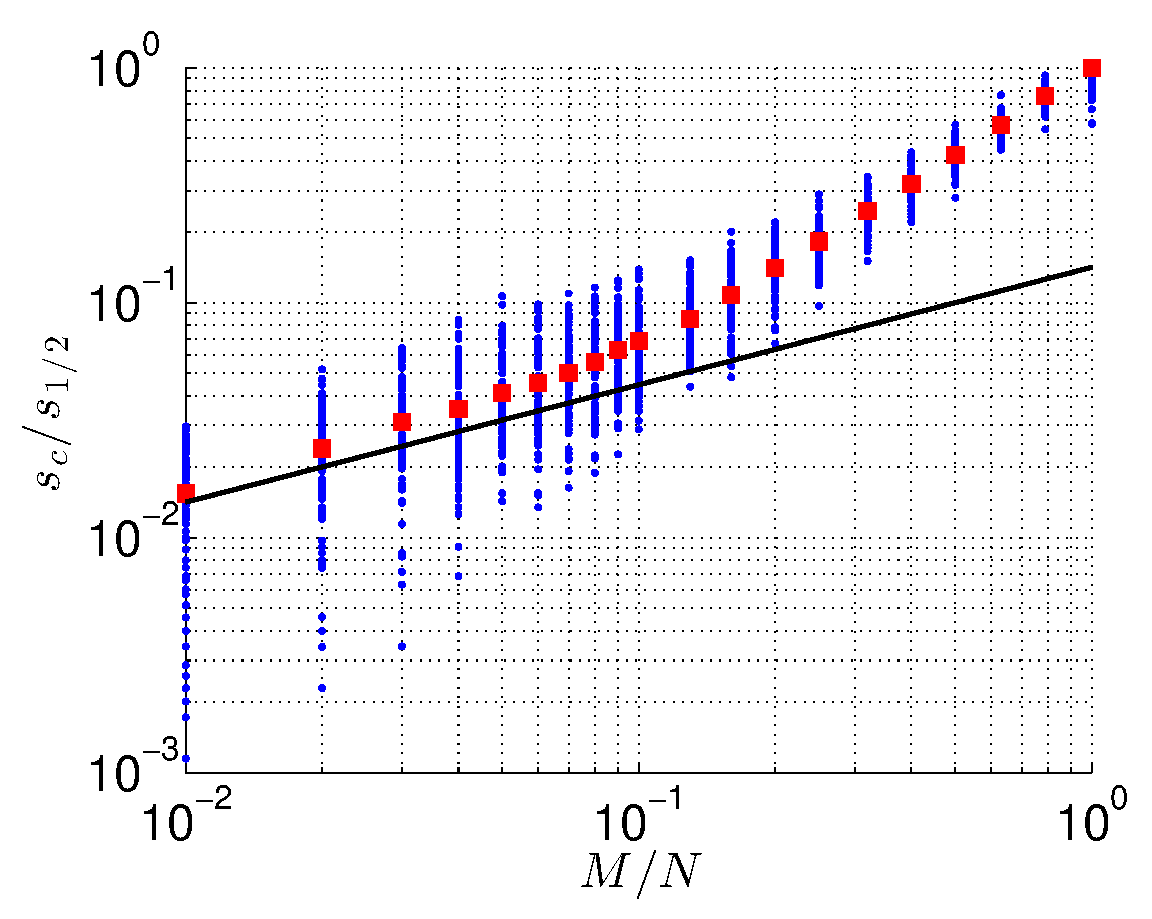
\includegraphics[height=5cm]{s_c_sparse_100_loglog}
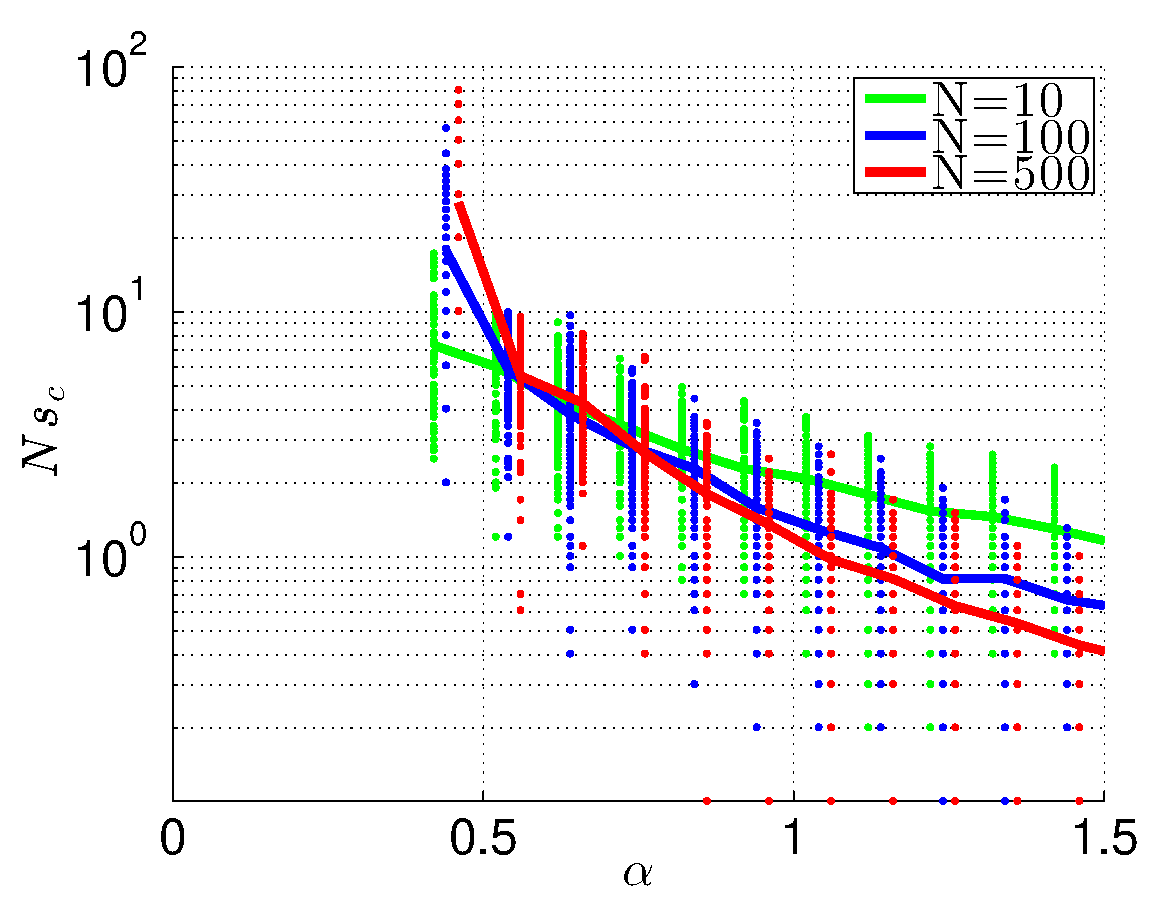
\includegraphics[height=5cm]{s_c_vs_alpha}

\caption{\label{figSc}
{\bf The complexity threshold.}
%
Top panel: The threshold value $s_c$ for delocalization versus the number of stochastic field defects $M$. 
The number of sites is $N{=}100$ and the disorder strength (of the defected sites) is $\sigma{=}5$. 
Blue dots correspond to different realizations, while red dots are the average (per~$M$). 
For a fully disordered lattice we expect $s_c=s_{1/2}$, hence the scaling of the axes. 
The black line is $s_c=\sqrt{M}\sigma/N$. %\Eq{e33}. 
%
Bottom panel: The threshold value~$s_c$ versus~$\alpha$. 
The dots are for different realizations, while the lines are the statistical average.  
For ${\alpha<1/2}$ the $s_c$ diverges as $N$ is increased.  
Data points for each $N$ are slightly shifted for clarity.
}
\end{figure}



% Saturation
%%%%%%%%%%%%%%%%%%%%%%%%%
\begin{figure}
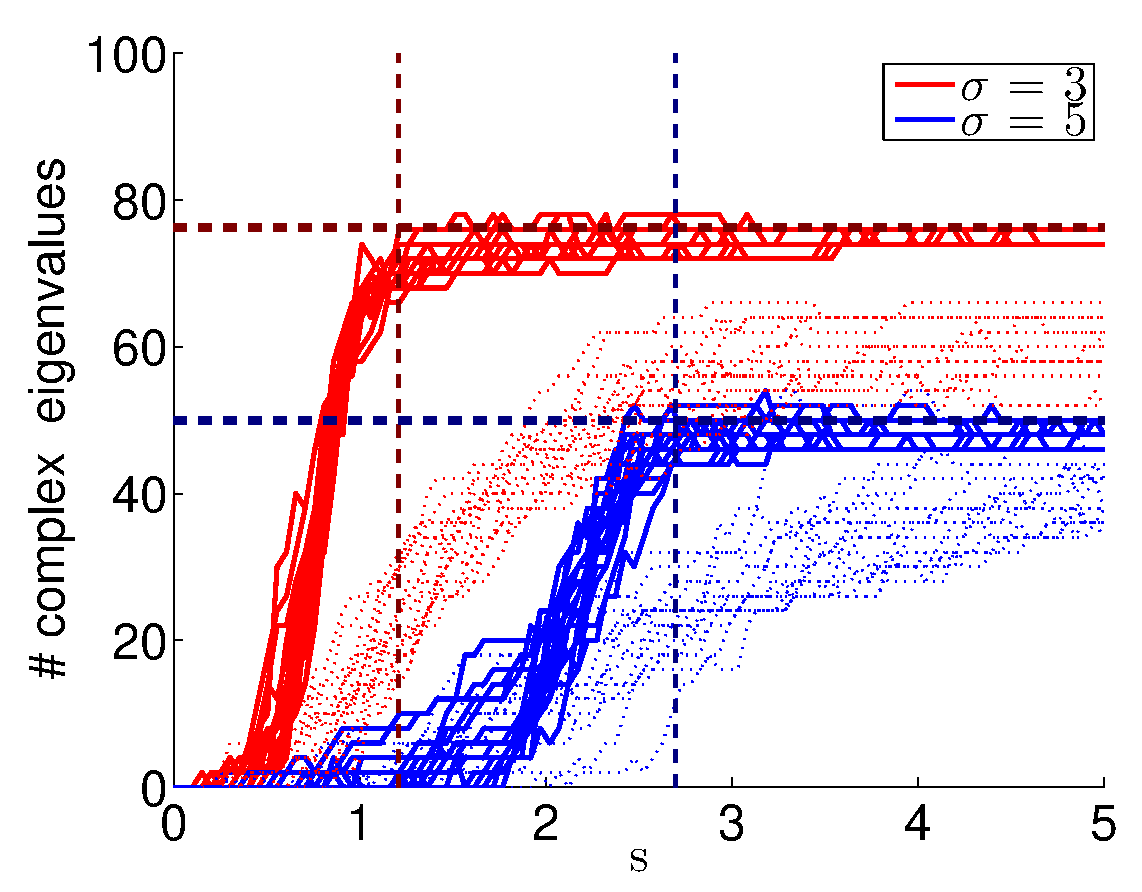
\includegraphics[height=5.4cm]{numComplex_100_alpha_sigma}

\caption{\label{figCplxSat}
{\bf Complexity saturation.}
The number of complex eigenvalues is counted for a ring with $N{=}100$ sites, 
for various values of the affinity~$s$. Each red line corresponds to a different
realization of field disorder with $\sigma{=}3$ (red) and $\sigma{=}5$ (blue). 
The vertical lines are the corresponding values of~$s_1$, 
at which the sliding transition occurs. 
We see that the asymptotic fraction of complex eigenvalues saturates. 
The horizontal dashed line are the analytical estimates of \Eq{e101}. 
If the lattice were continuous with Gaussian disorder, 
the number of complex eigenvalues would go to~$100\%$.
In the background a disordered resistor network with ${\alpha=0.9}$ is shown. 
The crossover is blurred and the saturation value is lower compared to \Eq{e101}.  
}
\end{figure}






%%%%%%%%%%%%%%%%%%%%%%%%%%%%%%%%%%%%%
\sect{Electrostatic picture}
%
In order to get an insight into the secular equation we 
define an ``electrostatic" potential by taking the log 
of the left hand side of \Eq{e20}. Namely, 
%
\be{22}
\Psi(z) \ \ = \ \ \sum_k \ln\left(z-\epsilon_k\right) \ \ \equiv \ \ V(x,y)+iA(x,y)
\eeq
%
where ${z=x+iy}$. Note that we have flipped the sign convention (${z\mapsto -z}$), 
and also we set the time units such that $\overline{w}=1$.
% 
The constant ${V(x,y)}$ curves correspond to potential contours,
and the constant ${A(x,y)}$ curves corresponds 
to stream lines. The derivative $\Psi'(z)$ corresponds to the field, 
which can be regarded as either electric or magnetic field up to a 90deg rotation.       
Using this language, the secular equation takes the form
%
\be{21}
V(x,y)=V(0); \ \ \ \ A(x,y)=2\pi*\text{integer} 
\eeq
%
Namely the roots are the intersection of the field lines with the 
potential contour that goes through the origin (\Fig{froots}). 
%
%
We want to find what are the conditions for getting 
a real spectrum from \Eq{e21}, and in particular what 
is the threshold $s_c$ for getting complex eigenvalues 
at the bottom of the spectrum. 
We first look on the potential along the real axis:
%
\be{23}
V(\epsilon) \ \ = \ \  \int \ln \left(|\epsilon-x' \right|) \rho(x')dx' 
\eeq
%
In regions where the $\{\epsilon_k\}$ form a quasi-continuum,  
one can identify $(1/N)V(\epsilon)$ as the Thouless expression  
for the inverse localization length \cite{Shnerb1}.
The explicit value of $V(0)$ is implied by \Eq{e20}, 
namely ${V(0)=\ln[2(\cosh(S_{\circlearrowleft}/2)-1)]}$.   
For a charge-density that is given by \Eq{e3}, with some cutoff $\epsilon_c$,
the derivative of the electrostatic potential at the origin is (see Methods)
%
\be{19}
V'(\epsilon) \approx  \frac{ \epsilon^{\mu-1}}{\epsilon_c^{\mu}} \pi \mu \cot(\pi \mu)
\eeq
%
One observes that the sign changes from positive to negative at $\mu=1/2$.
Some examples are illustrated in \Fig{froots}.
Clearly, if the envelope of $V(\epsilon)$ is above 
the $V=V(0)$ line, then the spectrum is real, and the $\lambda_k$ are roughly 
the same as the $\epsilon_k$, shifted a bit to the left. 


From the above it follows that the threshold~$s_c$ 
for the appearance of a complex quasi-continuum 
is either  ${V(\epsilon_s)<V(0)}$  or  ${V'(0)<0}$, 
depending on whether $\varrho(\epsilon)$ is gapped or not. 
In the latter case it follows from \Eq{e19} that ${s_c=s_{1/2}}$.
%
We note that for the Gaussian model of \cite{odh3}
one obtains ${V(\epsilon \rightarrow \infty) = \text{const}}$,  
implying that the entire spectrum would go from real to complex at $s=s_{1/2}$. 
In general this is not the case: the complex spectrum typically 
forms a ``bubble" tangent to the origin, or possibly 
one may find some additional bubbles as in \Fig{froots}b.   


The identification of the~$s_c$ with $s_{1/2}$ holds for full disorder, 
but not for sparse disorder. In the latter case ${s_c \propto 1/N}$, 
or we may better look on ${S_c=Ns_c}$. 
The reasoning that leads to this conclusion is as follows: 
We start with a clean ring. Recall that $\varrho(\epsilon)$ 
feature a gap ${[0,\epsilon_s]}$. If we have $M$ uncorrelated defected 
bonds with some $\sigma$ disorder the condition ${V(\epsilon_s)<V(0)}$
implies ${S_c=\sqrt{M}\sigma}$ (see methods).
The handling of weak links is a bit more complicated (see Methods)
but leads to the same conclusion, where the role of $\sigma$ 
is played by the dispersion of the defected~$w_n$.     
  



%%%%%%%%%%%%%%%%%%%%%%%%%%%%%%%%%%%%%%
\sect{Complexity saturation}
%
The secular equation for the eigenvalues is given by \Eq{e20}.
%
In the nonconservative case, the eigenvalues of $\bm{H}$ do not depend on $s$,
thus raising $s$ will eventually make the entire spectrum complex. 
For a conservative matrix, however, $V(\epsilon)$ is also a function of $s$, 
so increasing $s$ raises $V(\epsilon)$  at the same rate.
%
Taking $s$ to be as large as desired, the eigenvalues of~$H$ 
become trivially $\gamma_{n}\eexp{\mathcal{E}_n/2}$, 
and the equation $V(\epsilon)=V(0)$ for the upper cutoff $\epsilon_c$ 
of the complex energies takes the form
%
\be{24}
\overline{\ln\left[ \epsilon - w\eexp{\mathcal{E}/2} \right]} \ \ = \ \ s/2 
\eeq
%
It is natural to write the stochastic field as $\mathcal{E}=s+\varsigma$, 
such that ${\varsigma\in[-\sigma,+\sigma]}$. 
For the purpose of presentation we assume that~$w{=}1$.  
Then the spectrum stretches from $\epsilon_s=\eexp{(s-\sigma)/2}$ 
to ${\epsilon_c=\eexp{(s+\sigma_c)/2}}$,  
where $\sigma_c$ is the solution of
%
\beq
\int_{-\sigma}^{\sigma} \ln \left| \eexp{{\varsigma}/2} - \eexp{\sigma_c /2}\right| d\varsigma  \ \ = \ \ 0 
\eeq
% 
It follows that the fraction of complex eigenvalues is 
%
\be{101}
\text{fraction} 
= \frac{1}{N}\int_{\epsilon_s}^{\epsilon_c} \rho(\epsilon) d\epsilon
= \frac{1}{\sigma}\ln\left( \frac{\epsilon_c}{\epsilon_s} \right) 
= \frac{\sigma_c + \sigma}{2\sigma}
\eeq
%
We demonstrate the agreement with this formula in \Fig{figCplxSat}.
We plot there also what happens if resistor-network disorder is introduced.
We see that for small~$\alpha$ the crossover is not as sharp and 
the saturation value is lower than \Eq{e101} as expected from \Eq{e24}. 


%\newpage
%%%%%%%%%%%%%%%%%%%%%%%%%%%%%%%%%%
\sect{In conclusion}  
we have shown that the relaxation properties of a closed circuit (or chemical-cycle), 
whose dynamics is generated by a conservative rate-equation,  
is dramatically different from that of a biased non-hermitian Hamiltonian. 
The transition to complexity depends on the type of disorder as summarized in table \ref{tbl}. 
Surprisingly it happens for ${\alpha>1/2}$ before the percolation transition, 
and for ${\mu>1/2}$ before the sliding transition, and diminishes as $1/N$ for sparse disorder.
Further increasing the bias does not lead to full delocalization, instead a ``complexity saturation" is observed.





% DOS
%%%%%%%%%%%%%%%%%%%%%%%%%%%%%%
\begin{figure}
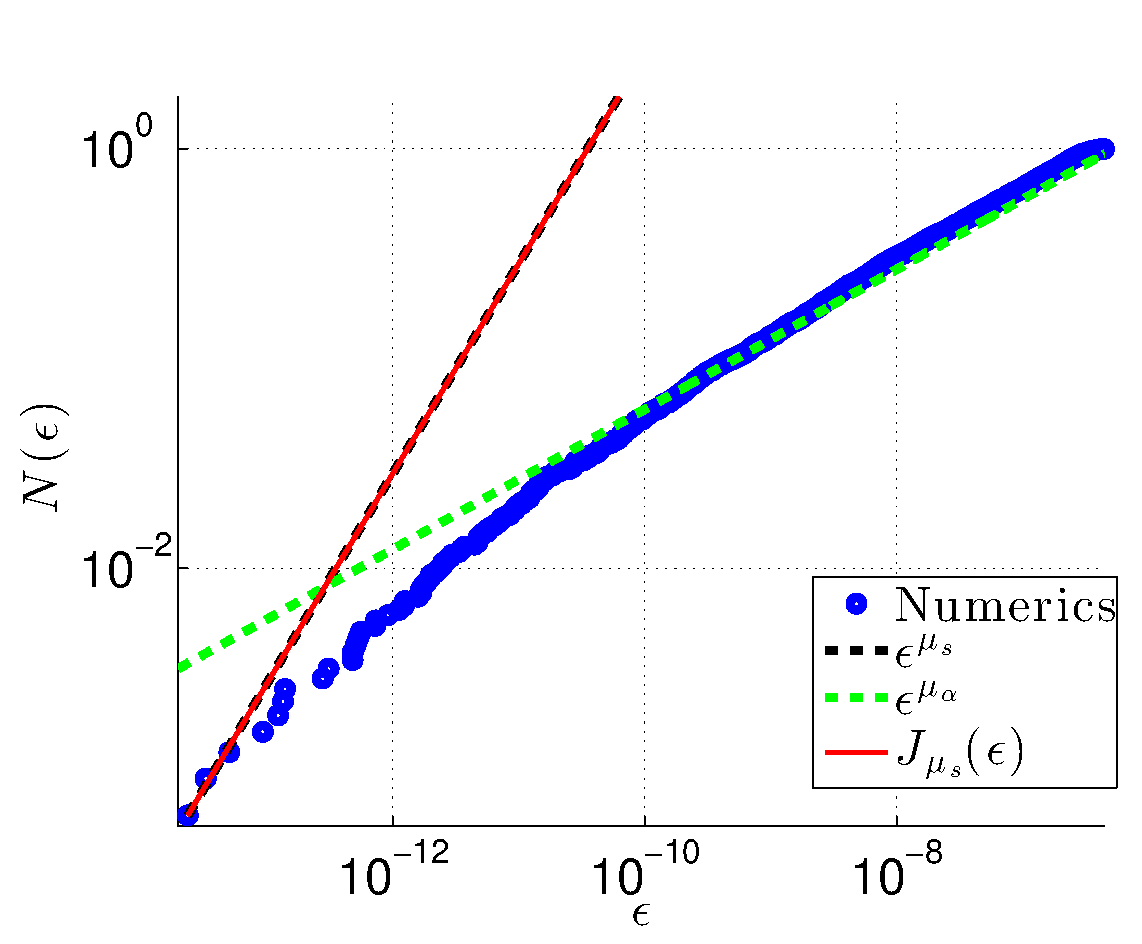
\includegraphics[height=5cm]{N_E_1_1_french}

\caption{\label{fdos}
{\bf The spectrum of the associated hermitian matrix.}
We calculate numerically the integrated density, 
which counts the eigenvalues ${\{\epsilon_k<\epsilon\}}$ of $\bm{H}$ 
for a ring with $N{=}3000$ sites. 
The system is characterized by a percolation exponent ${\mu=\mu_{\alpha}=1/3}$, 
and by a scaled affinity ${\mu=\mu_s=1}$. 
The stochastic-field distribution is with $\sigma{=}2$. 
The blue points are are results of numerical diagonalization. 
There is a crossover from density that corresponds to $\mu_s$ (dashed black line), 
to density that corresponds to $\mu_{\alpha}$ (dashed green line). 
The red line is the Bessel expression of \cite{odh3}. 
}
\end{figure}




%%%%%%%%%%%%%%%%%%%%%%%%%%%%%%%%%%%%%%%%%%%%%%%%%%%%%%%%%%%%%%%%%%%%%%%%%%
%%%%%%%%%%%%%%%%%%%%%%%%%%%%%%%%%%%%%%%%%%%%%%%%%%%%%%%%%%%%%%%%%%%%%%%%%%
\section{Methods}  

%%%%%%%%%%%%%%%%%%%%%%%%%%%%%%%%%%%%%%%%%%%%%%%%%%%%%%%%%%%%%%%%%%%%%%%%%%
\sect{The percolation threshold}
%
An example where the percolation issue arises is provided by 
the analysis of relaxation in ``glassy" networks \cite{ege,egt}, 
where the sites are distributed randomly in space, 
and the rates depend exponentially on the inter-site distance, 
namely ${w \propto \exp(-r/\xi)}$. 
In such type of model there is a percolation-related crossover 
to variable-range-hopping \cite{pts}. But in one-dimension
there is a more dramatic crossover to sub-diffusion \cite{Alexander}.
The statistics of the inter-site distances is Poisson ${\text{Prob}(r) \propto \exp(-r/a)}$, 
where $a$ is the mean spacing, and therefore ${\alpha=\xi/a}$ in \Eq{e5}.     
The diffusion coefficient is the harmonic average over~$w$, 
reflecting serial addition of connectors. It becomes zero for ${\alpha<1}$. 


%%%%%%%%%%%%%%%%%%%%%%%%%%%%%%%%%%%%%%%%%%%%%%%%%%%%%%%%%%%%%%%%%%%%%%%%%%
\sect{The NESS formula}
%
Following the derivation in \cite{nes} the explicit formula for the NESS is   
%
\beq
p_n \ \propto \ \left( \frac{1}{w_{\overrightarrow{n}}}\right)_s e^{-\left(U(n)-U_s(n)\right)}
\eeq
%
where $U(n)$ is the stochastic potential that is associated with the field $\mathcal{E}_n$, 
the transitions in the drift-wise direction are $w_{\overrightarrow{n}}=w_n\eexp{\mathcal{E}_n/2}$, 
and the subscript~$s$ indicates drift-wise smoothing over a length scale~$1/s$. 
Note that in the absence of bias the smoothed functions are constant and we get the canonical equilibrium state.    
\\


%%%%%%%%%%%%%%%%%%%%%%%%%%%%%%%%%%%%%%%%%%%%%%%%%%%%%%%%%%%%%%%%%%%%%%%%%%
\sect{The similarity transformation}
%
Define the diagonal matrix $\bm{U}=\mbox{diag}\{U(n)\}$. 
The stochastic field can be made uniform, as in \cite{Shnerb1}, 
by performing a similarity transformation ${\tilde{\bm{W}} = \eexp{{\bm{U}/2}} \bm{W} \eexp{-{\bm{U}/2}}}$,  
leading to 
%
\be{16}
\tilde{\bm{W}} \ = \ 
\text{diagonal}\Big\{-\gamma_{n}\Big\} 
+\text{offdiagonal}\Big\{  w_{n}\eexp{\pm \frac{S_{\circlearrowleft}}{2N}}  \Big\}
\eeq
%
where the "$\pm$" are for the forward and backward transitions respectively.
Note that the $s$-dependent statistics of the~$\mathcal{E}_n$ is still hiding in the diagonal elements.
The associated symmetric matrix $\bm{H}$ is defined by setting ${S_{\circlearrowleft}=0}$.
Then one can define an associated spectrum ${\epsilon_k}$.
For an open chain setting ${S_{\circlearrowleft}=0}$ can be regarded 
as a gauge transformation of an imaginary vector potential.
For a closed ring ${S_{\circlearrowleft}}$ is like an 
imaginary Aharonov-Bohm flux, and cannot be gauged away. 
\\

%%%%%%%%%%%%%%%%%%%%%%%%%%%%%%%%%%%%%%%%%%%%%%%%%%%%%%%%%%%%%%%%%%%%%%%%%%
\sect{Finding $s_{\mu}$}
%
The cummulant generating function of the stochastic field 
can be written as $g(\mu)=(s-s_{\mu})\mu$,  
where the $s_{\mu}$ are defined via the following expression:   
%
\be{362}
\left\langle  e^{-\mathcal{E}\mu}\right\rangle \ \ \equiv \ \ \eexp{-(s-s_{\mu})\mu} 
\eeq
%  
If the stochastic field has normal distribution 
with standard deviation $\sigma$, then ${s_{\mu}=(1/2) \sigma^2 \mu}$.
For our log-box distribution \Eq{e5} applies. 
The finite value of $s_{\infty}$ reflects that $\mathcal{E}$ is bounded.  
\\

%%%%%%%%%%%%%%%%%%%%%%%%%%%%%%%%%%%%%%%%%%%%%%%%%%%%%%%%%%%%%%%%%%%%%%%%%%
\sect{Finding $V'(0)$}
%
To derive \Eq{e19} we assume an integrated density of states that corresponds to \Eq{e3}, 
namely, ${\mathcal{N}(\epsilon) = (\epsilon/\epsilon_c)^{\mu}}$, 
where $\epsilon_c$ is some cutoff that reflects the discreteness of the lattice.
After integration by parts the electrostatic potential along the real axis is given by 
%
\beq
V(\epsilon) \ \ = \ \ -  \int_0^{\epsilon_c} \frac{\mathcal{N}(x)}{x-\epsilon}dx
\eeq
%
While calculating the derivative we assume ${\epsilon \ll \epsilon_c}$, 
hence taking the upper limit of the scaled integral as infinity: 
%
\beq
V'(\epsilon) \ \ &=& \ \ 
\frac{\mu}{\epsilon_c^{\mu}} \epsilon^{\mu-1} \int_0^{\infty} \frac{z^{\mu-1}}{z-1}dz 
\\
&=&   
-\frac{\mu}{\epsilon_c^{\mu}}  \epsilon^{\mu-1} \ B_{\infty}(\mu,0)
\eeq  
%
where $B_u(a,b)$ is the Incomplete Euler Beta function.
Taking the Cauchy principal part we get
%
\beq
B_{\infty}(\mu,0) &=&  
\lim_{\delta \to 0}  \left[ B_{1-\delta}(\mu,0) - B_{1-\delta}(1-\mu,0) \right]  
\\
&=& \psi(1-\mu)-\psi(\mu) = \pi \cot(\pi \mu)
\eeq
%
where $\psi(z)$ is the digamma function,
and the last equality has been obtained by the reflection formula. 
\\



% SecularEq for Ring with "g"
%%%%%%%%%%%%%%%%%%%%%%%%%%%%%%%
\begin{figure}

%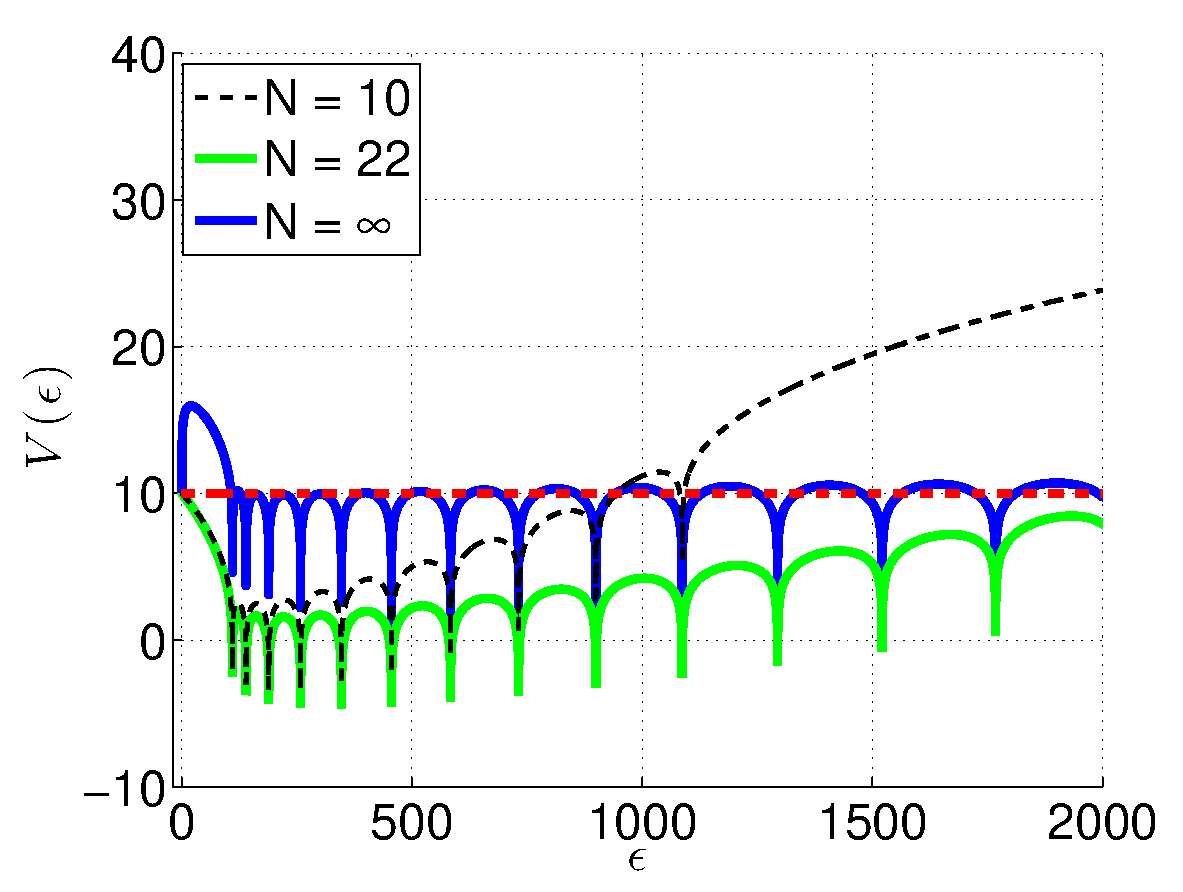
\includegraphics[height=5cm]{gRing_ES_vs_cont2}
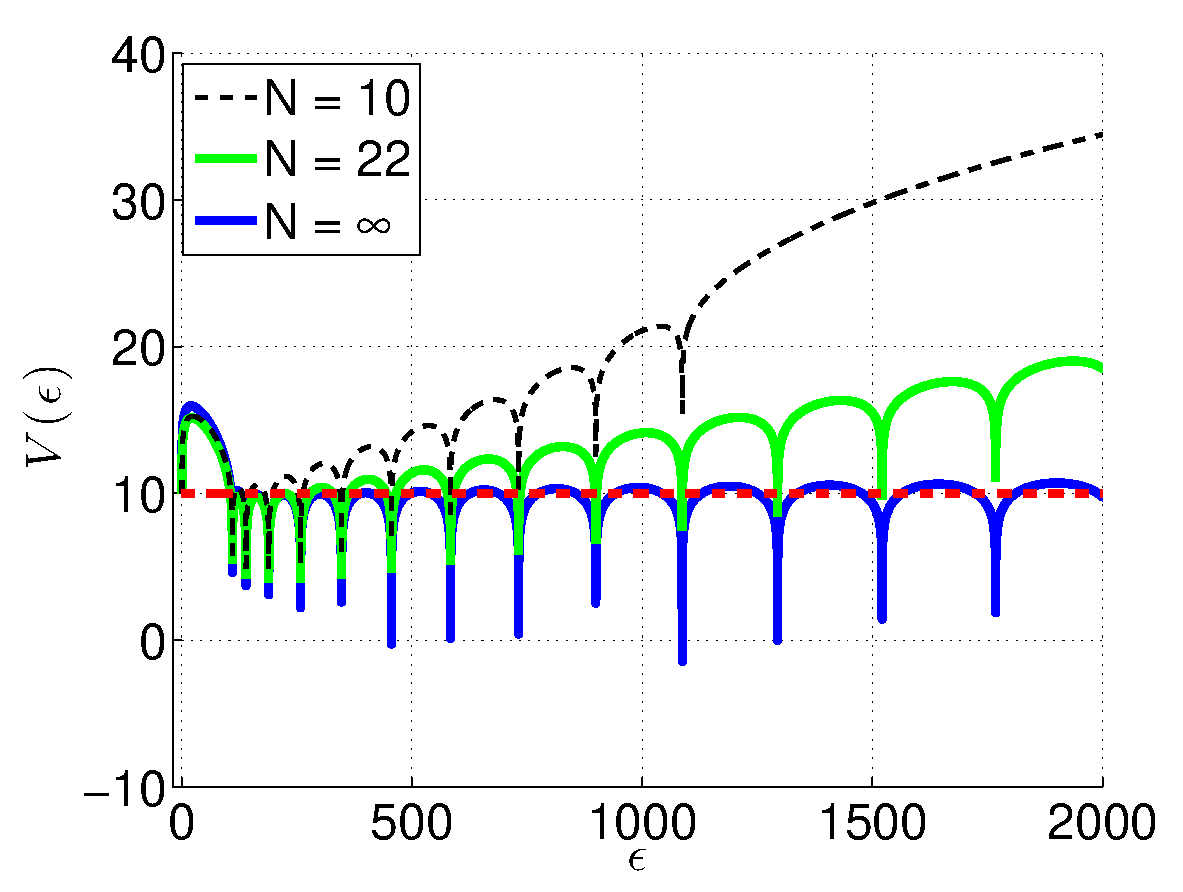
\includegraphics[height=5cm]{gRing_ES_vs_cont}

\caption{\label{figReconstruction} 
{\bf Graphical illustration of the the secular equation for a ring with a weak link.} 
The red line is $V(0)$.  
The blue line is $V(\epsilon)$ as deduced from the LHS of \Eq{e50}
with ${L=1}$, and ${g=10^{-3}}$ and ${S_{\circlearrowleft}=20}$.
The yellow line is an attempted reconstruction of $V(\epsilon)$ 
from the first $N=22$ roots $\epsilon_k$ of the $S_{\circlearrowleft}{=}0$ equation. 
The green line is a proper reconstruction that takes into account 
an impurity term $\epsilon_0$. The deviation from the blue line 
for large~$k$ is due to finite truncation: compare the ${N{=}10}$ line with the ${N{=}22}$ line. 
}
\end{figure}




%%%%%%%%%%%%%%%%%%%%%%%%%%%%%%%%%%%%%%%%%%%%%%%%%%%%%%%%%%%%%%%%%%%%%%%%%%
\sect{Finding $s_c$ due to a biased-link}
%
We consider a clean ring. We assume that the stochastic field 
over one bond is exceptionally large compared to all other bonds.   
Then there is an extra ``impurity" level  
${\epsilon_1 \approx \gamma_1 \approx \exp[(s+\sigma)/2]}$ 
that is located above the continuum of extended modes. 
The contribution of this impurity to $V(\epsilon_s)$ 
is $\ln(\epsilon_s-\gamma_1)$. 
The contribution of the continuum can be neglected 
due to the Thouless relation. 
Hence the condition ${V(\epsilon_s)>V(0)}$ 
implies $s_c \approx \sigma/N$. 
\\     


%%%%%%%%%%%%%%%%%%%%%%%%%%%%%%%%%%%%%%%%%%%%%%%%%%%%%%%%%%%%%%%%%%%%%%%%%%
\sect{Finding $s_c$ due to a weak-link}
%
We consider a clean ring of length ${L=Na}$ with lattice spacing $a$ 
and identical bonds (${w_n=1}$).  
We change one bond into a weak link (${w_1 \ll 1}$). 
This setup can be treated exactly in the continuum limit, 
where \Eq{e1} corresponds to a diffusion equation  
with coefficient ${D_0=wa^2}$ and drift velocity ${v_0=swa}$.  
The weak link corresponds to a segment 
where the diffusion coefficient is ${D_1 \ll D_0}$.  
Using transfer matrix methods we find the secular equation 
%
\be{50}
\cos(k) + \frac{1}{g} \frac{k^2+\left(\frac{S_{\circlearrowleft}}{2}\right)^2}{2k}\sin(k)
\ = \ \cosh \left(\frac{S_{\circlearrowleft}}{2} \right)
\eeq
%
where ${k^2= (L^2/D) z - (S_{\circlearrowleft}/2)^2}$, 
and $g=(D_1/a)/(D_0/L)$. We have taken here 
the limit ${a\rightarrow0}$, keeping~$(L,g,S_{\circlearrowleft})$ constant. 
The equation is graphically illustrated in \Fig{figReconstruction}. 
All the roots are real solutions provided the envelope 
of the left-hand-side (LHS) lays above the right-hand-side (RHS).
The minimum of the envelope of the LHS is obtained at ${z = S_{\circlearrowleft}^2/2}$.
Consequently we find that the threshold~$S_c$ obeys 
%
\be{23}
\frac{S_{\circlearrowleft}}{2g} \ \ = \ \ \cosh\left[ \frac{S_{\circlearrowleft}}{2} \right]
\eeq
%
provided $S_{\circlearrowleft} \gg g$, which is self-justified for small~$g$.   
The solution is given in terms of the Lambert function, 
namely ${S_c = -2 \mathbb{W}(-g/2)}$, leading to ${s_c=S_c/N}$.

 
The secular, equation \Eq{e50}, parallels the discrete version \Eq{e20}, 
with a small twist that we would like to point out.
Naively one would like to identify $\ln [2 (\text{LHS} -1)]$, 
up to a constant, with $\sum_{k=1}^{\infty} \ln(\epsilon-\epsilon_k)$, 
where the $\epsilon_k$ are the roots of \Eq{e50} with $S_{\circlearrowleft}{=}0$ 
in the RHS. This is tested in \Fig{figReconstruction}, 
and we see that there is a problem. Then one realizes 
that in fact an additional $k=0$ term with ${0 \lesssim \epsilon_0 < \epsilon_s}$ 
is missing. Going back to the discrete version it corresponds 
to an impurity-level that is associated with a mode which is located 
at the weak-link.
While taking the limit ${a\rightarrow0}$ this level becomes excluded.
Adding it back we we see that the agreement between \Eq{e20}      
and \Eq{e50} is restored. The residual systematic error as $k$ becomes 
larger is due to finite truncation of the number of roots used in the reconstruction. 
%
Making the approximation ${\ln(\epsilon_s-\epsilon_0) \approx \ln[(s/2)^2]}$,  
and noting that ${g\propto N}$, it is verified that the 
equation  ${V(\epsilon_s) = V(0)}$  for the complexity threshold 
is consistent with \Eq{e23}. 


%%%%%%%%%%%%%%%%%%%%%%%%%%%%%%%%%%%%%%%%%%%%%%%%%%%%%%%%%%%%%%%%%%%%%%%%%%%%%%%%%%%%
%%%%%%%%%%%%%%%%%%%%%%%%%%%%%%%%%%%%%%%%%%%%%%%%%%%%%%%%%%%%%%%%%%%%%%%%%%%%%%%%%%%%
%%%%%%%%%%%%%%%%%%%%%%%%%%%%%%%%%%%%%%%%%%%%%%%%%%%%%%%%%%%%%%%%%%%%%%%%%%%%%%%%%%%%
%%%%%%%%%%%%%%%%%%%%%%%%%%%%%%%%%%%%%%%%%%%%%%%%%%%%%%%%%%%%%%%%%%%%%%%%%%%%%%%%%%%%
\bibliography{neg}{}
\bibliographystyle{naturemag}


%%%%%%%%%%%%%%%%%%%%%%%%%%%%%%%%%%%%%%%%%%%%%%%%%%%%%%%%%%%%%%%%%%%%%%%%%%
%%%%%%%%%%%%%%%%%%%%%%%%%%%%%%%%%%%%%%%%%%%%%%%%%%%%%%%%%%%%%%%%%%%%%%%%%%

\onecolumngrid

\ \\ 

\sect{Acknowledgements}
%
This research has been supported by the Israel Science Foundation (grant No. 29/11). 
\\


\hidea{

\sect{Author contributions statement}
%
Both authors have contributed to this article. 
\\

\sect{Additional information} 
%
% Reprints and permissions information is available at www.nature.com/reprints\\
The authors declare that they have no competing financial interests.
% Correspondence and requests for materials should be addressed to dcohen@bgu.ac.il

}



A\]
\end{document}